\documentclass[main]{subfiles}
\begin{document}
\begin{figure}\resizebox{0.8\textwidth}{!}{%
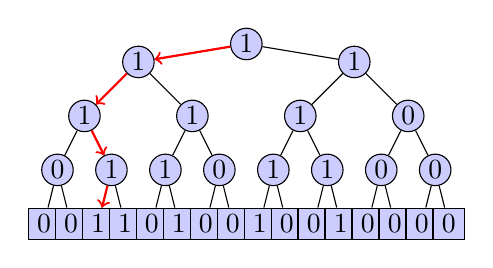
\begin{tikzpicture}[scale=0.65,
		level 1/.style={
			sibling distance=12em, level distance=1em,
			nodes={circle,inner sep=1pt, draw=black, fill=blue!20, minimum size=4mm}
		},
		level 2/.style={
			sibling distance=6em, level distance=3em,
			nodes={circle,inner sep=1pt, draw=black, fill=blue!20, minimum size=4mm}
		},
		level 3/.style={
			sibling distance=3em, level distance=3em,
			nodes={circle,inner sep=1pt, draw=black, fill=blue!20, minimum size=4mm}
		},
		level 4/.style={
			sibling distance=1.5em,
			nodes={rectangle,inner sep=1pt, draw=black, fill=blue!20, minimum size=4mm}
		},
	]
	\node [circle, inner sep=1pt, draw=black, fill=blue!20, minimum size=4mm] (a){$1$}
		child { node {$1$}
			child { node {$1$}
				child { node {$0$}
					child { node {$0$} }
					child { node {$0$} }
				}
				child { node {$1$} 
					child { node {$1$} }
					child { node {$1$} }
				}
			}
			child { node {$1$}
				child { node {$1$}
					child { node {$0$} }
					child { node {$1$} }
				}
				child { node {$0$}
					child { node {$0$} }
					child { node {$0$} }
				}
			}
		}
		child { node {$1$}
			child { node {$1$}
				child { node {$1$}
					child { node {$1$} }
					child { node {$0$} }
				}
				child { node {$1$}
					child { node {$0$} }
					child { node {$1$} }
				}
			}
			child { node {$0$}
				child { node {$0$}
					child { node {$0$} }
					child { node {$0$} }
				}
				child { node {$0$}
					child { node {$0$} }
					child { node {$0$} }
				}
			}
		};
		\draw[->,red,thick] (a) to (a-1);
		\draw[->,red,thick] (a-1) to (a-1-1);
		\draw[->,red,thick] (a-1-1) to (a-1-1-2);
		\draw[->,red,thick] (a-1-1-2) to (a-1-1-2-1);

\end{tikzpicture}
}
\caption{$\Min(V), V = \{2,3,5,8,11\}$}
\end{figure}
\end{document}

